% might need psfig, url, amsmath, amsfonts?
\documentclass[psfig]{acm_proc_article-sp}

\begin{document}

\title{StreaMIT: A Language for Streaming Applications\thanks{This
document is {\bf MIT/LCS Technical Memo}, August 2001.  A similar
version was submitted to POPL 2002.  Please do not distribute.}}

\numberofauthors{1}
\author{
\alignauthor Bill Thies, Michal Karczmarek, and Saman Amarasinghe\\
	\vspace{12pt}
	Laboratory for Computer Science \\
	Massachusetts Institute of Technology \\
	Cambridge, MA  02139 \\
	\vspace{12pt}
	{\tt \{thies, karczma, saman\}@lcs.mit.edu}
}

\date{today}

% for the arrow of a function def, etc.
\newcommand{\ma}[2]{max_{#1 \rightarrow #2}}
\newcommand{\mal}[1]{maxloop_{#1 \rightarrow #1}}
\newcommand{\mi}[2]{min_{#1 \leftarrow #2}}

\maketitle

\begin{abstract}
Due to the high data rates involved in audio, video, and signal
processing applications, it is imperative to compress the data to
decrease the amount of storage used.  Unfortunately, this implies that
any program operating on the data needs to be wrapped by a
decompression and re-compression stage.  Re-compression can incur
significant computational overhead, while decompression swamps the
application with the original volume of data.

In this paper, we present a program transformation that greatly
accelerates the processing of compressible data.  Given a program that
operates on uncompressed data, we output an equivalent program that
operates directly on the compressed format.  Our transformation
applies to stream programs, a restricted but useful class of
applications with regular communication and computation patterns.  Our
formulation is based on LZ77, a lossless compression algorithm
utilized by ZIP, and immediately applies to simpler formats such as
Apple Animation, Microsoft RLE, and Targa.

We implemented a simple subset of our techniques in the StreamIt
compiler, which emits executable plugins for two popular video editing
tools: MEncoder and Blender.  For common operations such as color
adjustment and video compositing, computing directly on compressed
data offers a speedup roughly proportional to the overall compression
ratio.  For our benchmark suite of 12 videos in Apple Animation
format, speedups range from 1.1x to 471x, with a median of 15x.

\end{abstract}

\section{Introduction}


Stream computing represents an increasingly important class of
applications. In streaming codes, there is an abundance of parallelism that
is easier to extract compared to traditional desktop workloads (e.g.,
pointer-based computing). As a result, the extraction of parallelism
in streaming codes does not require heroic efforts, and thus,
processors can deliver higher performance with significantly lower
power costs. This is especially important since
leading microprocessor companies have realized that modern general
purpose architectures are near their  performance limits for  the
amount of power they consume. Thus, the future will place a greater
emphasis on exploiting the properties of streaming workloads in
conventional von~Neumann architectures.

Streaming is a model of computation that uses sequences of data
and computation kernels to expose concurrency and locality for
efficiency~\cite{wss}. In general purpose processors, improving locality 
translates to an effective management of the memory hierarchy at all
levels, including the register file. In this paper, we present a
methodology for compiling streaming codes to general purpose,
cache-based architectures. We first introduce a simple model for
reasoning effectively about the caching behavior of streaming
workloads. This model serves as a foundation for several {\it cache-aware
optimizations} that are geared toward the concomitant increase of instruction
and data {\it temporal locality}. These
optimization lead to significantly better utilization of the memory
system, and as such, they deliver performance gains ranging from 11
to 99\% for our streaming benchmark suite.

The context for our work is StreamIt, an architecture-independent
language that is engineered for streaming
applications~\cite{streamitcc}. It adopts the 
Cyclo-Static Dataflow~\cite{BELP96} model of computation which is a
generalization of Synchronous Dataflow~\cite{LM87-i} (SDF).  
SDF is a popular  model that  is well suited for
streaming codes. In SDF, computation is represented as a graph
consisting of {\it  actors} connected by communication channels; the
actors consume  and produce a constant number  of items from their
input and output  channels every time they execute. SDF is appealing
because it is amenable to static scheduling and optimization. 

From a general purpose architecture's point of view, actors represent
computation kernels, and the communication between actors represents
data buffers that must be streamed to and from the processor. Thus
the size of an actor and the
order of actor executions are critical properties that
impact the performance of the instruction cache. For example, the
compiler must make sure the actor's code size is not
greater than the instruction cache. Furthermore, we must {\it scale}
the execution of the actor so that it runs several times before we move
on to some other actor in the stream 
graph. This serves to $(i)$ amortize the cost of fetching the actor's
instructions into the cache from memory (an expensive operation), $(ii)$
improve the instruction temporal locality, and $(iii)$ improve overall
performance. However, as our cache model will show, we 
cannot arbitrarily scale the execution frequency of an actor. This
is because actors produce data that must be buffered, and therefore,
we must also consider the amount of data an actor produces and
consumes if we are to adequately manage the data cache. This paper is unique
in that it is the first to present a unified optimization methodology
that simultaneously considers instruction and data locality for
mapping streaming computation to cache-based architectures.

In terms of improving the data cache behavior, the compiler schedules
actor firing such that the producer-consumer locality is
preserved. Furthermore,  the compiler may {\it fuse}
together two or more actors to form a coarser grained kernel.
The fusion allows for better register allocation as we can
destroy the arrays used to buffer data between the actors and replace
the corresponding array references with scalars.  It also allows for
various competing implementations for managing the buffers between the
fused actors.  This paper evaluates several implementation
alternatives (for buffer management) and evaluates their performance.

The methodology for fusing actors leverages a distinguishing StreamIt
characteristic, namely, the hierarchical organization of
the stream graph. Furthermore, the algorithm for fusing actors applies
for the various topologies allowed by StreamIt.
It also considers another distinguishing characteristics of StreamIt,
namely the {\tt peek} operation whereby an actor may inspect data
items in its input buffer without consuming them until some future
execution. While peeking is a powerful language feature, it does pose
some challenges to the compiler and the cache optimizations. Peeking
also impacts the choice for the best buffer management strategy, as our
study will show.

%% the comment about p3 and itanium not being embedded architectures
%% is out of the blue! need a better transition.
Cache-aware fusion alone delivers significant performance gains, although our
evaluation shows that fusion with scaling leads to the best
performance on a general purpose, cache-based architecture. For our
experiments, we use two different processors: a superscalar out-of-order
processor, and an in-order VLIW processor. The former is a Pentium~3
whereas the latter is an Itanium~2. While these architectures are not
particularly suited for an embedded system, they do exhibit some
properties that are worthy of investigation. Furthermore, that we can
demonstrate measurable performance gains on real systems is far more
convincing than using a simulation-based environment. We chose the
Pentium~3 processor because it has very few registers in its
instruction set architecture. The Itanium by contrast has a much 
larger and richer repertoire of registers. The two architectures serve
to validate our cache-aware optimizations, in that we expect an
architecture with more register to benefit more from optimization such
as scalar replacement. On average, fusion leads to a 47\% improvement
on the Pentium~3, and 50\% on the Itanium~2.

The two architectures also differ in terms of their memory system
organization. The Itanium is an in-order VLIW processor and does not
tolerate a memory stall as well as its out-of-order
counterpart. Therefore we expect different gains from the scaling
optimization which amortize the long access latencies for instruction
and data caches. On average, scaling leads to a 21\% improvement on
the Itanium~2, and 17\% on the Pentium~3.

While both scaling and fusion lead to modest performance gains, we
must combine the two to deliver the best possible performance. When we
do so, we can further improve the performance of our benchmarks by
53\% on average for the Pentium~3, and 55\% for the Itanium~2.

\subsection{Summary of Contributions}

This paper makes the following contributions:
\begin{itemize}

\item A cache model for stream computing that provides a quantitative
estimate of the caching performance for any sequence of actor
executions.

\item A cache-aware scheduling heuristic that judiciously increases
the multiplicity of actors, improving instruction and data locality
while not exceeding the data cache.

\item A cache-aware partitioning policy that judiciously fuses
adjacent actors into a single component, enabling local optimizations
while not exceeding the instruction cache.

\item An optimized buffer management policy, termed ``copy-shift with
execution scaling'', which out-performs a traditional rotating buffer
in a detailed micro-benchmark analysis.

\item A fully automatic implementation of the above techniques in the
StreamIt compiler.

\item An experimental evaluation across 11 streaming benchmarks,
demonstrating performance improvements of up to 99\%.
\end{itemize}

\subsection{Paper Roadmap}

The remainder of the paper is organized as follows. Section~\ref{sec:streamit}
describes StreamIt and introduces our motivating example.
Section~\ref{sec:cache-model} introduces our cache model for 
reasoning about the performance of a streaming
computation. Section~\ref{sec:cache-opt} describes our cache-aware
optimizations, and Section~\ref{sec:buffer} describes the 
optimization enabled by fusion. Section~\ref{sec:evaluation} describes
our evaluation methodology and present our experimental
analysis. Sections~\ref{sec:related-work}~and~\ref{sec:conclusion}
discuss related work and concludes the paper.

\section{Streaming Application Domain}
\label{sec:domain}

The applications that make use of a stream abstraction are diverse,
with targets ranging from embedded devices, to consumer desktops, to
high-performance severs.  However, we have observed a number of
properties that these programs have in common--enough so as to
characterize them as belonging to a distinct class of programs, which
we will refer to as {\it streaming applications.}  The following are
the salient properties of a streaming application, independent of its
implementation:
\begin{enumerate}

\item {\it Large streams of data.}  Perhaps the most fundamental
aspect of a streaming application is that it operates on a large (or
virtually infinite) sequence of data items, hereafter referred to as a
{\it data stream}.  Data streams generally enter the program from some
external source, and each data item is processed for a limited time
before being discarded.  This is in contrast to scientific
applications, in which a fixed input set is manipulated with a large
degree of data reuse.

\item {\it Independent stream filters.}  Conceptually, a streaming computation
represents a sequence of transformations on the data streams in the
program.  We will refer to the basic unit of this transformation as a
{\it filter}: an operation that--on each execution step--reads one or
more items from an input stream, performs some computation, and writes
one or more items to an output stream.  Filters are generally
independent and self-contained, without references to global variables
or other filters.  A stream program is the composition of filters into
a {\it stream graph}, in which the outputs of some filters are
connected to the inputs of others.

\item {\it A stable computation pattern.}  The structure of the stream
graph is generally constant during the steady-state operation of a
stream program.  That is, a certain set of filters are repeatedly
applied in a regular, preditable order to produce an output stream
that is a given function of the input stream.

\item {\it Occaisional re-initialization.}  Even though each
arrangement of filters is executed for a long time, there are still
dynamic modifications to the stream graph that occur on occaision.
For instance, if a wireless network interface is experiencing high
noise on an input channel, it might react by adding some filters to
clean up the signal; a software radio re-initializes a portion of the
stream graph when a user switches from AM to FM.  Sometimes, these
re-iniitializations are synchronized with some data in the stream--for
instance, when a network protocol changes from bluetooth to 802.11 at
a certain point of a transmisison.  There are typically an ennumerable
number of configurations that the stream graph can adopt in any one
program, such that all of the possible arrangments of filters are
known at compile time.

\item {\it Occaisional out-of-stream communication.}  In addition to
the high-volume data streams passing from one filter to another,
filters also communicate small amounts of control information on an
infrequent and irregular basis.  Examples include changing the volume
on a cell phone, printing an error message to a screen, or changing a
coefficient in an upstream FIR filter.

\item {\it High performance expectations.}  Often there are real-time
constraints that must be satisfied by streaming applications; thus,
efficiency (in terms of both latency and throughput) is of primary
concern.  Additionally, many embedded applications are intended for
mobile environments where power consumption, memory requirements, and
code size are also important.

\end{enumerate}



 






\section{Language Overview}

\begin{figure}[t]
\scriptsize
\begin{verbatim}
Example FIR / FFT goes here.
\end{verbatim}
\vspace{-12pt}
\caption{\protect\small FIR / FFT Filters.
\protect\label{fig1}}
\vspace{-12pt}
\end{figure}

In this section, we give an overview of the StreaMIT language.

\begin{verbatim}

- motivated by properties above
- this is interface language; developing higher-level streamit
- legal java syntax for now, to ease development cycle

- point to example, talk through major features

---------------------------------------------------------------------------
- representing filters 
- others:
	- procedural language
		- complicated loops that don't express well the feedback,
			parallelism in streaming systems
		-> loop overhead dominates, data leaves the cache

	- object oriented language
		- complicated runtime-model, pulling data and trying to 
			get block size right for machine configuration
			(scheduling is complicated)

- us: only define base-level blocks, leave the rest to language/compiler
	- init, work, message handlers

	- define in init function anything that has to be set up when
          the block is first defined.

	- define in work function the finest-grained step of
          execution, expressing the simple transfer function of one
          stream into another

	- no global data or global time

- syntax presented:  filter/channel declarations, init & work functions
---------------------------------------------------------------------------
- representing streams (how to ``connect the blocks together'')
- others:
	- straight-line code declaring & connecting blocks
		problem: can't see the structure.
			 easy to make mistakes
	- ad-hoc graph languages for declaring & connecting blocks
		problem: awkward to use
			 no good textual representation

	  generally, arbitrary connections are too hard to think
		about. and too hard for compiler to analyze.
		make connection with unstructured control flow

- us: structured streams.
	- compose out of simple structures:  
		pipe, feedbackloop, splitjoin

	   advantages: can see structure in code, with indentation
		level corresponding to hierarchical stream
		depth (pointer to natural syntax argument?)

		- can have clean abstractions about *hierarchical*
		structure.  Provides better abstraction and
		modularity than *flat* layout of blocks.

- syntax presented:  stream, feedbackloop, splitjoin.  inlining.
---------------------------------------------------------------------------
- integrated support for infrequent, low-bandwidh messages
- others:
	- embed control messages in data stream
		- complicated, error-prone, unreadable code
		- hurts performance of steady state (if you have to 
			check if everything is message or data)
		- complicates compiler analysis
		- can't send messages upstream without explicit
			feedback loop
	- treat messages as synchronous method calls
		- but delays stream progress when method en route, 
			disrupting scheduling freedom of compiler, as
			well as efficiency when at time of call
		- usually there is no return value (it's a message!)
		- no good notion of ``when'' message arrives relative
			to sender
- us: 	- support for asynchronous messages with timing relative to
		data items
	- (define the ``wavefront'' of a data item, and say that
		messages sent with range of times)
	- avoids problems of two above approaches (it's readable, out
		of the way of steady-state data, and out of way of compiler)
	- this RELATIVE time gives more freedom to compiler for
		scheduling blocks
	- absence of global time good for parallel programming

- syntax presented:  sendMessage, messageHandlers, messageStubs.
---------------------------------------------------------------------------
- integrated support for re-initialization sections of a stream
- others:	
	- ad-hoc halting of whole stream's data flow so that some
		restructuring can take place
		
		- complicated programming to interface between the time of
			reinitialization and starting/stopping the stream

- us:
	- re-invoke the original initialization routine with different 
		parameters.

		- talk about draining the pipeline.  the compiler
                  worries about doing the reinitialization at the
                  right time so that the re-initialized segment drains
                  completely.  but the re-init message is delivered
                  just like a message, and a warning is given if the
                  message delivery schedule does not encompass a clean
                  draining point.

		- (alternatively, could destroy the pipeline.)

		- so improvement #1 is that the interface to the user is 
			cleaner.  Also it's easier for the compiler to 
			analyze.

		- improvement #2: very clear targets of
			re-initiailization.  Can reinitialize any
			block in the hierarchy in a very well-defined
			way.

		- improvement #3 is that the draining analysis is done
                  automatically, which otherwise is very complicated
                  for the programmer to deal with.

- syntax presented:  special reset method

\end{verbatim}







\section{Semantics of Time}

In this section we develop a more formal semantics for the message
delivery guarantees described above.  The timing model in StreaMIT is
unique in that all time is relative to {\it information
wavefronts}--that is, two independent filters can describe a common time
only in terms of when the {\it effects} of one filter's execution are
seen by another.  Thus, although each filter's {\tt work} function is
invoked asynchronously without any notion of global time, two
invocations of a work function occur at the same ``information-relative
time'' if they operate on the same information wavefront.

To define this notion more precisely, we present transfer functions
that describe the flow of information across filters and streams.
Using these transfer functions, we translate message delivery
constraints into a set of constraints on the execution schedule of the
stream graph.  Finally, we use these scheduling constraints to
formulate an operational semantics for messaging and latency in
StreaMIT.

\subsection{Information Flow}

The concept of information flow is central to the streaming domain.
When an item enters a stream, it carries with it some new information.
As execution progresses, this information cascades through the stream,
effecting the state of filters and the values of new data items which
are produced.  We refer to an ``information wavefront'' as the
sequence of filter executions that first sees the effects of a given
input item.  This wavefront is well-defined even in the presence of
rate-changing filters that peek or pop a different number of items
than they push.

\begin{figure}
\centering
\psfig{figure=Tapes.eps,width=3.2in}
\caption{fig1}
\label{fig:tapes}
\end{figure}

To formalize the wavefront, we introduce some new representations for
the state of the stream graph.  Consider that in place of each data
channel there is an infinite ``tape'' which contains the history of
values that have been pushed onto the channel (see Figure
\ref{fig:tapes}).  Now consider the following functions:

\begin{itemize}

\item Given that there are $x$ items on tape $a$, the maximum number
of items that can appear on tape $b$ is $\ma{a}{b}(x)$.

\item Given that there are $x$ items on tape $b$, the minimum number
of items that must appear on tape $a$ is $\mi{a}{b}(x)$.

\end{itemize}

Note that these functions are only defined over pairs of tapes $(a,
b)$ where $a$ is ``upstream'' of $b$--that is, where there is a
directed path in the stream graph from the filter following $a$ to the
filter preceding $b$.

The $max$ and $min$ functions are related to the information wavefront
in the following sense.  The item at position $y = \mi{a}{b}(x)$ of
tape $a$ is the latest item on tape $a$ to {\it affect} the item at
position $x$ of tape $b$.  This is because item $x$ on tape $b$ can be
produced if and only if tape $a$ contains at least $y$ items.  Note
that this effect might be via a control dependence rather than a data
dependence--for instance, if item $y$ needed to pass through a
round-robin joiner before some data from another stream could be
routed to tape $b$.

We now turn to deriving expressions for $\ma{a}{b}$ and $\mi{a}{b}$ as
a step towards formalizing the semantics of messaging and latency in
StreaMIT.

\subsubsection{Filters}

Consider a filter $A$ that peeks $peek_A$, pops $pop_A$, and pushes
$push_A$ data items on every execution step.  Further, let us denote
the input and output tapes of $A$ by $I_A$ and $O_A$, respectively.
We now turn our attention to finding $\ma{I_A}{O_A}$ and
$\mi{I_A}{O_A}$, describing the transfer of information across the
filter $A$.

To derive $\ma{I_A}{O_A}(x)$, observe that the filter can execute so
long as it does not peek beyond the $x$'th item on the input tape,
$I_A$.  After the $n$'th execution, it has popped $n$ items, peeked up
to $n + (peek_A - pop_A)$, and popped $2 * n$ items.  Thus, it can
execute $n = \lfloor(x - (peek_A - pop_A)) / pop_A)\rfloor$ times, leaving
the following expression for $\ma{I_A}{O_A}(x)$

\[
\begin{array}{l}
\ma{I_A}{O_A}(x)  \\ 
\makebox[.1in]{ } = \left\{
\begin{array}{ccl}
push_A*\left\lfloor\frac{x-(peek_A-pop_A)}{pop_A}\right\rfloor & if & x \ge (peek_A-pop_A) \\
 & \\
0 & if & x < (peek_A-pop_A) \\
\end{array} \right.
\end{array}
\]


\subsubsection{Pipelines}

Let us now derive expressions for $min$ and $max$ in the case of
pipelined filters.  In the base case, consider that two filters are
connected, with the output of $A$ feeding the input of $B$.  We are
seeking $\ma{I_A}{O_B}(x)$: the maximum number of items that can
appear on tape $O_B$ given that there are $x$ items on tape $I_A$.
Observing that a maximum of $\ma{I_A}{O_A}(x)$ items can appear on
tape $O_A$, and that $O_A$ must equal $I_B$ since the filters are
connected, we see that a maximum of
$\ma{I_B}{O_B}(\ma{I_A}{O_A}(x))$ items can appear on $O_B$:
\begin{equation*}
\ma{I_A}{O_B} = \ma{I_B}{O_B} \circ \ma{I_A}{O_A}
\end{equation*}
In the case of $\mi{I_A}{O_B}(x)$, the order of composition is
reversed: given that there are $x$ items on tape $O_B$, a minimum of
$\mi{I_B}{O_B}(x)$ are on tape $I_B$, and since $O_B = I_A$, we have
that a minimum of $\mi{I_A}{O_A}(\mi{I_B}{O_B}(x))$ items appear on
$I_A$, leaving:
\begin{equation*}
\mi{I_A}{O_B} = \mi{I_A}{O_A} \circ \mi{I_B}{O_B}
\end{equation*}
By identical reasoning, these composition laws hold for pipelined
streams as well as filters.  That is, given tapes $x$, $y$, and $z$, 
we have that:
\begin{eqnarray}
\label{eq:compose}
\ma{x}{z} = \ma{y}{z} \circ \ma{x}{y} \\
\mi{x}{z} = \mi{x}{y} \circ \mi{y}{z}
\end{eqnarray}
However, there are some restrictions on these definitions.  They only
apply when there is a downstream path $P_1$ from the filter following
$x$ to the filter preceding $y$, a downstream path $P_2$ from the
filter following $y$ to the filter preceding $z$, and the paths $P_1$
and $P_2$ are non-overlapping.  This restriction prevents the
successive composition of transfer functions around feedback loops,
thereby ensuring a unique definition for all pairs $(x, z)$ where
there is a downstream path from $x$ to $z$.

\subsubsection{SplitJoins}

\begin{figure}
\centering
\psfig{figure=splitjoin.eps,width=3.2in}
\caption{\protect\small SplitJoin Construct with labeling.
\protect\label{splitjoin}}
\end{figure}

We now derive $min$ and $max$ in the case of a SplitJoin, as pictured
in Figure {\ref:splitjoin}.  For the splitter $S$ there are two output
tapes; let us denote them by $O1_S$ and $O2_S$.  Similarly, let us
denote the two input tapes of the joiner $J$ by $I1_J$ and $I2_J$.  We
now derive the transfer functions for round robin and
duplicate/combine nodes.  Note that the duplicate/combine nodes can be
simulated with round robins and duplicating filters, but we provide
the transfer functions anyways to simplify the semantic analysis of a
program.

{\bf Round robin splitter.}  In the case of a round-robin splitter, the
items from the input tape are alternately routed to the output tapes,
with the first item going onto tape $O1_S$.  By this definition, we
can see that the splitter's $max$ is defined as follows:
\begin{eqnarray*}
\ma{I_S}{O1_S}(x) = \left\lceil\frac{x}{2}\right\rceil \\
\ma{I_S}{O2_S}(x) = \left\lfloor\frac{x}{2}\right\rfloor
\end{eqnarray*}
To derive the $min$ function across a splitter, observe that the input
tape need only progress so far as to produce the items on the emptier
output tape.  That is, we need to consider the number of items on both
of the splitter's output to determine the minimum number of items that
are needed at its input.  Thus, our $min$ function has two arguments:
the first corresponding to $O1_S$ and the second corresponding to
$O2_S$.  The equation is as follows:
\begin{eqnarray*}
\mi{I_S}{(O1_S, O2_S)}(x_1, x_2) = min(2*x_1-1, 2*x_2)
\end{eqnarray*}
{\bf Round robin joiner.}  The rules for a round robin joiner are in
some sense dual to those of the round robin splitter.  Again assuming
that items are alternately drawn from the input tapes, starting with
$I1_J$, we have that:
\begin{eqnarray*}
\mi{I1_J}{O_J}(x) = \left\lceil\frac{x}{2}\right\rceil \\
\mi{I2_J}{O_J}(x) = \left\lfloor\frac{x}{2}\right\rfloor
\end{eqnarray*}
Again, the $max$ function takes two arguments, corresponding to the
number of items on $I1_J$ and $I2_J$, respectively:
\begin{eqnarray*}
\ma{(I1_J, I2_J)}{O_J}(x_1, x_2) = min(2*x_1-1, 2*x_2)
\end{eqnarray*}
{\bf Duplicate splitter}.  Clearly, the $max$ function of a duplicate
splitter is simply the identity function, since it maps each element
on the input tape to the same location on the output tapes:
\begin{eqnarray*}
\ma{I_S}{O1_S}(x) = x \\
\ma{I_S}{O2_S}(x) = x
\end{eqnarray*}
The $min$ function is similar, except that--like the round robin
split--the input need only progress as far as the lesser output:
\begin{eqnarray*}
\mi{I_S}{(O1_S, O2_S)}(x_1, x_2) = min(x_1, x_2)
\end{eqnarray*}
{\bf Combine joiner.} The combine joiner is simply the dual of the
duplicate splitter, with transfer functions that the reader can verify
as follows:
\begin{eqnarray*}
\ma{(I1_J, I2_J)}{O_J}(x_1, x_2) = min(x_1, x_2) \\
\mi{I1_J}{O_J}(x) = x \\
\mi{I2_J}{O_J}(x) = x
\end{eqnarray*}

\subsubsection{FeedbackLoops}

\begin{figure}
\centering
\psfig{figure=feedback.eps,width=3.2in}
\caption{\protect\small  FeedbackLoop construct labeling.
\protect\label{looplabel}}
\end{figure}

We have to be careful when defining the transfer functions for
feedback loops (see Figure {\ref:looplabel}).  The feedback splitter
$FS$ serves as a normal splitter, and has the same $min$ and $max$
functions as defined above.  However, the feedback joiner $FJ$ is
slightly different than a standard joiner, since during the first few
executions it fabricates values from the loop body before they appear
on the input tape.  The transfer function must take special account of
these initial values, since they are never appear on $I2_{FJ}$, the
input tape from the loop body.  This is because we model the
initialization of FeedbackLoops by feeding the joiner the initial
values directly instead of pushing them onto a channel.

Recall that if the feedback loop specifies a wavefront latency of $n$,
then $n$ initial values are provided to the feedback joiner before
values from the feedback loop are read.  Assume that the round robin
feedback joiner first draws from the data stream $I1_J$, and then from
the feedback loop $I2_J$.

The $min$ function for the main stream is as before:
\begin{eqnarray*}
\mi{I1_J}{O_J}(x) = \left\lceil\frac{x}{2}\right\rceil 
\end{eqnarray*}
However, the equation must include the initial $n$ values for the
$min$ function of the loop:
\begin{eqnarray*}
\mi{I2_J}{O_J}(x) = \left\lfloor\frac{x}{2}\right\rfloor - n
\end{eqnarray*}
The $max$ function must be similarly shifted for the input from the loop:
\begin{eqnarray*}
\ma{(I1_J, I2_J)}{O_J}(x_1, x_2) = min(2*x_1-1, 2*(x_2+n))
\end{eqnarray*}

\subsubsection{Summary}

We have derived expressions for $\ma{a}{b}$ and $\mi{a}{b}$ for when
$a$ and $b$ are the respective input and output to 1) a filter, 2) a
pipeline, 3) a split or join, and 4) a feedback split or join.  By
composing these expressions following Equation~\ref{eq:compose}, we
can arrive at values of $\ma{a}{b}$ and $\mi{a}{b}$ for all pairs of
tapes $(a, b)$ where there is some directed path through the stream
graph--that is, along the direction of data flow--from the filter
reading from tape $a$ to the filter writing to tape $b$.

\subsection{Semantics}

Equipped with definitions of $\ma{a}{b}$ and $\mi{a}{b}$, we can now
address the semantics of StreaMIT's message delivery and latency
guarantees.

\subsubsection{Messages}

Suppose that filter $A$ sends a message to filter $B$ with latency
$n$, where $n$ is any integer.  In $n$ invocations of $A$'s {\tt work}
function, $A$ will produce one or more data items $d$.  Now, the
messaging system guarantees that:

\begin{enumerate}

\item If $B$ is upstream of $A$, then $B$ will receive the message
immediately following the last invocation of its {\tt work} function
which produces items that affect $d$.

\item If $B$ is downstream of $A$, then $B$ will receive the message
immediately preceding the first invocation of its {\tt work} function
which produces items that are effected by $d$.

\item If $B$ runs in parallel with $A$, then the message is in terms
of a shared set of splitters and joiners.  {\bf Flesh out details.}

\end{enumerate}

These guarantees can be expressed more formally as a set of
constraints on the number of items on certain tapes in the system.
Again, suppose that filter $A$ sends a message to filter $B$ with
latency $n$, where $n$ could is any integer.  Let $s$ denote the
number of items on $O_A$ when the message was sent, and $r$ denote the
number of items on $O_B$ when the message is received.  We have that:

\begin{enumerate}

\item If $B$ is upstream of $A$, the message will be delivered when:
\begin{eqnarray}
\label{eq:msgup}
r = \mi{O_B}{O_A}(s + push_A * n)
\end{eqnarray}
That is, $s + push_A * n$ is the number of items on $A$'s output tape
after producing the data of interest.  Then, $y =
\mi{O_B}{O_A}(s + push_A * n)$ is the latest item on $B$'s output
tape that affects the data of interest.  The message should be
delivered immediately after the work funtion producing this item,
which occurs when the item count $r$ equals $y$, as specified by the
constraint.

\item If $B$ is downstream of $A$, the message will be delivered when:
\begin{eqnarray}
\label{eq:msgdown}
r = \ma{O_A}{O_B}(s + push_A * (n-1))
\end{eqnarray}
That is, $s + push_A * (n - 1)$ is the number of items on $A$'s
output tape before pushing the data of interest, and $y =
\ma{O_A}{O_B}(s + push_A * (n-1))$ is the maximum number of items
on $B$'s output tape as a result of the outputs of $A$.  Thus, when
$A$ pushes the next set of data, it could affect the data that will be
pushed next onto the output tape of $B$.  (Note that the next set of
data from $A$ might not be sufficient to calculate the next set on
$B$'s output, but it could affect it nonetheless.)  The message must
be delivered immediately before this effected data appears on $B$'s
output, so the number of items $r$ on $B$'s output must equal $y$.

\end{enumerate}

\subsubsection{Latency}

\subsubsection{Scheduling}

We can fully define the possible sequences of filter executions as a
set of constraints on the number of items on each tape in the stream
graph.  This is useful not only from the perspective of semantics, but
for compiler analysis of the space of valid schedules.  We will use
$n(t)$ to represent the number of items on tape $t$ at a given point
of execution.  A configuration C of the stream graph can be completely
represented by the vector $(n(t_1), n(t_2), \dots, n(t_k))$, where
$t_1$ through $t_k$ are the tapes in the graph.  A legal configuration
must satisfy three sets of constraints:

\begin{enumerate}

\item {\it Data dependences.}  A filter can only have as many items on
its output tape as can be produced by the items on its input tape.
For each filter $A$ in the program, we have the constraint:
\begin{eqnarray*}
n(O_A) \le \ma{I_A}{O_A}(n(I_A))
\end{eqnarray*}
Equivalently, we can pose this constraint in the opposite direction:
each input tape must contain at least the number of items that are
required by the output tape:
\begin{eqnarray*}
n(I_A) \ge \mi{I_A}{O_A}(n(O_A))
\end{eqnarray*}

\item {\it Message guarantees.}  Suppose that a filter $A$ might send
a message to filter $B$ with a maximum latency of $l$ during any
invocation of its work function.  Then we must constrain the execution
of $B$ to make sure that it is not too far ahead to receive the
message with the given latency.  That is, we can only execute $B$ so
long as $n(O_B)$--the item count on its output tape--does not exceed
the count when a message would be delivered.  Recalling the expression
for message delivery time (Equations \ref{eq:msgup} and
\ref{eq:msgdown}), this constraint is as follows if $B$ is upstream of $A$:
\begin{eqnarray*}
n(O_B) \le \mi{O_B}{O_A}(n(O_A) + push_A * l)
\end{eqnarray*}
and as follows if $B$ is downstream of $A$:
\begin{eqnarray*}
n(O_B) \le \ma{O_A}{O_B}(n(O_A) + push_A * (n-1))
\end{eqnarray*}

\item {\it Latency guarantees.}

\end{enumerate}

{\bf Defining the schedule.}  For a stream graph with a given set of
latency requirements and message delivery guarantees, we now have a
set of constraints expressing whether or not a given configuration
$(n(t_1), n(t_2), \dots, n(t_k))$ is legal.  It is a straightforward
step to formulate a legal sequence of transitions between
configurations, thereby exactly defining a legal order in which to
execute the filters' work functions.

When the program begins, no items have been pushed on any data
channels.  Thus, each tape is empty, and the starting configuration
$C_0$ is simply the zero-vector.  It is possible that the initial
configuration violates some of the constraints imposed by the
messaging and latency constructs, in which case the compiler can
inform the programmer that the delivery constraints requested in the
program are unsatisfyable.

Let {\cal P}(C) denote whether or not the constraints for a stream
graph are satisfied for a given configuration C.  We can then write
the transition function between configurations as follows:
\begin{eqnarray*}
(n(t_1), \dots , n(out_A), \dots, n(t_k)); \\ \frac{{\cal P}((n(t_1), \dots , n(out_A + push_A), \dots, n(t_k)))}{(n(t_1), \dots , n(out_A + push_A), \dots, n(t_k))}
\end{eqnarray*}
To understand this rule, observe that if we execute one step of filter
$A$, the only difference between the original configuration $C$ and
the new configuration $C'$ is that the item count for the output tape
of $A$ has increased by $push_A$ in $C'$.  Thus, if $C$ was valid and
$C'$ satisfies the constraints {\cal P}, then $C'$ represents a legal
configuration and the execution of $A$ is valid.  These operational
semantics are interesting in that we do not need to explicitly model
which data items are currently in which channels; instead, all of the
state is captured in terms of each filter's execution history.

\subsection{Program Verification}

A number of program analysis techniques are also enabled by the $min$
and $max$ functions that we have defined.  In particular, it is very
simple to compute 1) whether or not the program will deadlock as a
result of a starved input channel, and 2) whether or not any buffer
will grow without bound during the steady-state execution of the
program.

{\bf Deadlock detection.}  The deadlock detection algorithm takes
advantage of the fact that the only loops in our stream graph are part
of a FeedbackLoop construct.  A stream graph will be deadlock-free if
and only if there is no net change of output rate in the feedback
loop.  This can be formulated in terms of the $max$ function by
requiring that the wavefront from the output of the feedback joiner
$FJ$ unto itself is the identity function.  However, since we were
careful to leave the $max$ function undefined over cycles in the
stream graph, we define a new function $maxloop$ that maps a given
feedback joiner to the information wavefront around the loop:
\begin{eqnarray*}
\mal{FJ}(x) \equiv \ma{I2_FJ}{O_FJ} \circ \ma{O_FJ}{I2_FJ}
\end{eqnarray*}
The order of composition is as in Equation \ref{eq:compose} for the
composition of pipelines. Also, for the purposes of calculating
$\mal{FJ}$, one must assume that there are an infinite number of items
on tape $I1_FJ$; that is, the join from the feedback loop is not
limited by the external data source.  

Finally, we can state the constraint that the feedback loop must
respect.  For a loop with declared latency $n$, the loop will neither
overflow nor deadlock if:
\begin{eqnarray*}
\mal{FJ}(x) = x + n
\end{eqnarray*}
If $\mal{FJ}(x)$ is less than $x + n$, then there will be deadlock in
the program.

{\bf Overflow detection.}  There are two places that a buffer can
overflow in the stream graph.  The first is in a feedback loop, when
$\mal{FJ}(x)$ (calculated above) is more than $x$.  The second case is
when the parallel streams of a split/join have different production
rates.  For a splitter $S$ and a joiner $J$, the production rates will
cause an overflow if and only if $\ma{O1_S}{I1_J}(x) -
\ma{O2_S}{I2_J}(x)$ is not $O(1)$.  This difference could be analyzed
by a compiler for every SplitJoin in the stream graph to verify that
no buffers will overflow during steady-state execution.




\section{Detailed Example}
\label{sec:example}

% dzm: this figure might just need to go.
\begin{figure*}
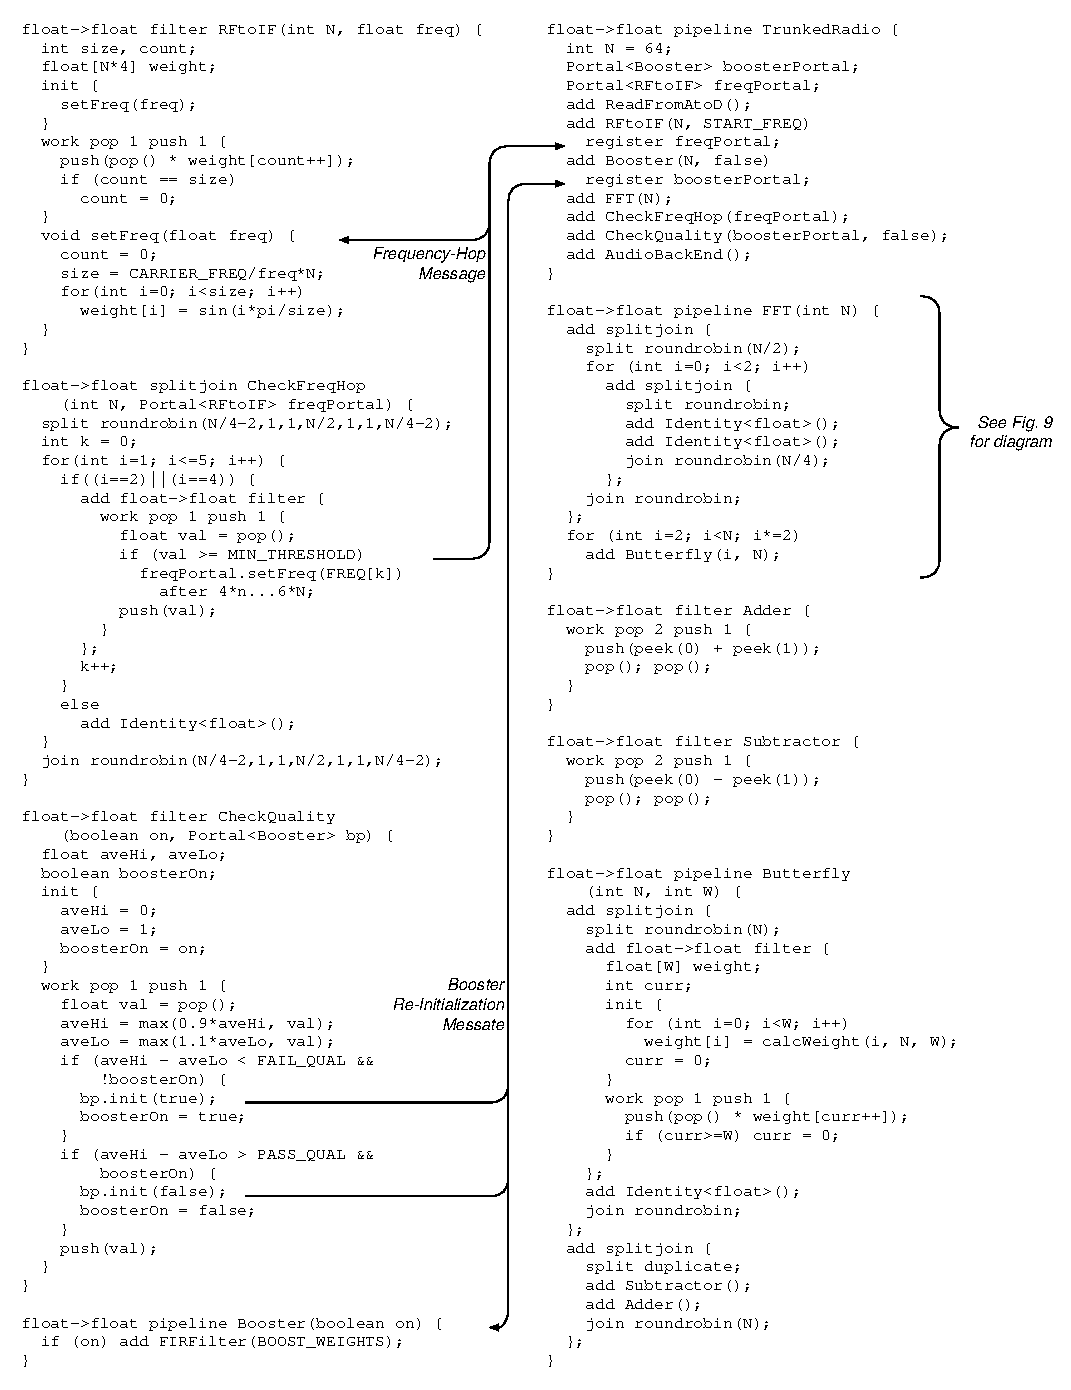
\includegraphics[width=\textwidth]{code-fm.eps}
\caption{StreamIt code for a software radio.  Arrows denote the paths
  of messages.}
\label{fig:radiocode}
\end{figure*}

We now discuss the StreamIt implementation of the Trunked Radio
illustrated in Fig.~\ref{fig:radiodiagram}.  The Trunked Radio is a
frequency-hopping system in which the receiver switches between a set of
known frequencies whenever it hears certain tones from the transmitter.

The toplevel class, \texttt{TrunkedRadio}, is implemented as a
seven-stage pipeline (see Fig.~\ref{fig:radiocode}).  The
\texttt{RFtoIF} stage modulates the input signal from RF to a
frequency band around the current IF frequency.  To support a change
in the IF frequency when frequency hopping occurs, the \texttt{RFtoIF}
filter contains a \texttt{setFreq} method that is invoked via a
message from the \texttt{CheckFreqHop} stage.  The message is sent
from \texttt{CheckFreqHop} with a latency range of $4N$ to $6N$, which
means that \texttt{RFtoIF} must deliver between $4N$ and $6N$ items
using the old modulation scheme before changing to the new frequency.

The optional \texttt{Booster} stage provides amplification for weak
signals, but is usually turned off to conserve power.  The
\texttt{Booster} is toggled by a re-initialization message from the
\texttt{CheckQuality} stage, which estimates the signal quality by the
shape of the frequency spectrum.  If all the frequencies have similar
amplitudes, \texttt{CheckQuality} assumes that the signal-to-noise
ratio is low and sends a message to activate the \texttt{Booster}.
This message is sent using best-effort delivery.

The \texttt{FFT} stage converts the signal from the time domain to the
frequency domain; please refer to p.~796 of \cite{clr} for a diagram
of the parallel FFT algorithm.  The StreamIt implementation consists
of a bit-reversal permutation followed by a series of
\texttt{Butterfly} stages.  The bit-reversal phase illustrates how
data can be reshuffled with just a few SplitJoin constructs (see
Fig.~\ref{fig:bitreverseorder}).  The \texttt{Butterfly}
stage--which is parameterized to allow for a compact representation of
the FFT--also employs split-joins to select groups of items for its
computation.  We believe that the StreamIt version of the FFT is clean
and intuitive, as the SplitJoin constructs expose the natural
parallelism of the algorithm.

%%% Local variables:
%%% TeX-master: "paper.tex"
%%% End:

\section{Related Work}
\label{sec:related}

% BILL

%Signal~\cite{Signal}, 
%Lucid~\cite{Lucid77}, and
%Occam~\cite{Occam}, and Sisal \cite{sisal}.
%Parallel Haskell~\cite{ph}
In addition to StreamIt, there are a number of stream-oriented
languages drawing from domains such as functional, dataflow, CSP and
synchronous programming~\cite{survey97}.  The Brook language is
architecture-independent and focusses on data
parallelism~\cite{brook04}.  Stream kernels are required to be
stateless, though there is special support for reducing streams to a
single value.  Stream\-C/Ker\-nel\-C is lower level than Brook;
kernels written in KernelC are stiched together in StreamC and mapped
to the data-parallel Imagine processor~\cite{imagine03ieee}.  SPUR
adopts a similar decomposition between ``microcode'' stream kernels
and skeleton programs to expose data parallelism~\cite{spur05samos}.
Cg exploits pipeline parallelism and data parallelism, though the
programmer must write algorithms to exactly match the two pipeline
stages of a graphics processor~\cite{cg03}.  Compared to these
languages, StreamIt places more emphasis on exposing task and pipeline
parallelism (all the languages expose data parallelim).
%and on sliding window operations (filters that peek).  
By adopting the synchronous dataflow model of execution~\cite{lee87},
StreamIt focusses on well-structured programs that can be aggressively
optimized.  The implicit infinite loop around programs is also a key
StreamIt characteristic that enables the transformations in this
paper.  Spidle is also a recent stream language that was influenced by
StreamIt~\cite{spidle03}.
%and Lucid Synchrone~\cite{Lucid-Synchrone}.
%Synchronous languages which
%target embedded applications include Esterel~\cite{Esterel},
%Lustre~\cite{Lustre}, and Additional

Liao et al. map Brook to multicore processors by leveraging the affine
partitioning model~\cite{liao06brook}.  While affine partitioning is a
powerful model for parameterized loop-based programs, in StreamIt we
simplify the problem by fully resolving the program structure at
compile time.  This allows us to schedule a single steady state using
flexible, non-affine techniques (e.g., simulated annealing) and to
repeat the found schedule for an indefinite period at runtime.
Gummaraju and Rosenblum map stream programs to a general-purpose
hyperthreaded processor~\cite{gummaraju05micro}.  Such techniques
could be integrated with our spatial partitioning to optimize per-core
performance.  Gu et al. expose data and pipeline parallelism in a
Java-like language and use a compiler analysis to efficiently extract
coarse-grained filter boundaries~\cite{du03sc}.  Ottoni et al. also
extract decoupled threads from sequential code, using hardware-based
software pipelining to distribute the resulting threads across
cores~\cite{ottoni05decoupled}.  By embedding pipeline-parallel
filters in the programming model, we focus on the mapping step.

%%%%%%%%%%%%%%%%%%%%%%%%%%%%%%%%%%%%%%%%%%%%%%%%%%%%%%%%%%%%%%%%%%%%%

Previous work in scheduling computation graphs to parallel targets has
focused on partitioning and scheduling techniques that exploit task
and pipeline parallelism~\cite{SDFSched, SDFSched2,may87communicating,
DAGSched, pipeline-sdf}.  Application of loop-conscious
transformations to coarse-grained dataflow graphs has been
investigated.  Unrolling (or ``unfolding'' in this domain) is employed
for synchronous dataflow (SDF) graphs to reduce the initiation
interval but they do not evaluate mappings to actual
architectures~\cite{unfolding,unfolding2}. Software pipelining
techniques have been applied to SDF graphs onto various embedded and
DSP targets~\cite{bakshi99,chatha-02}, but has required programmer
knowledge of both the application and the architecture. To our
knowledge, none of these systems automatically exploit the combination
of task, data, and pipeline parallelism.  Furthermore, these systems
do not provide a robust end-to-end path for application
parallelization from a high-level, portable programming language.

%% Previous work on instruction-level software pipelining has focused
%% mostly on scheduling machine instructions in a loop via modulo
%% scheduling~\cite{rau81,lam-softpipe}.  The algorithms devised must
%% account for tight resource constraints and complex instruction
%% dependences. Our software-pipelining problem is much less constrained,
%% enabling us to employ a simple greedy heuristic.  

%% Furthermore, a traditional modulo scheduling algorithm is not needed
%% because we have an implicit loop barrier at the end of each
%% steady-state.  ILP compilers for clustered VLIW
%% architectures~\cite{Bulldog,Multiflow,lee98spacetime,qian02} must
%% partition instructions and assign them to clusters as part of the
%% instruction scheduling. Clustering is analogous to our application of
%% filter fusion in our software pipelining algorithm.

\section{Conclusion}
\label{sec:conclusion}

In this paper, we describe the StreamIt compiler for the Raw
architecture.  The stream graph of a StreamIt program exposes the data
communication pattern to the compiler while the lack of global
synchronization frees the compiler to radically reoganize the program
for efficient execution on the underline architecture. The StreamIt
compiler demonstrates the power of this flexibility by totally
reoganizing large programs for better load balance. We were able to
map many of programs on to the Raw processor and obtain good
performance.

We introduce a collection of optimizations, vertical and horizontal
filter fusion, vertical and horizontal filter fission and filter
reordering transformations, that can be used to restructure stream
graphs.  We show that by applying these transformations we can map a
high-level stream program, written to reflect the composition of the
application, onto Raw and achieve good processor utilization and load
balance, leading to a factor of three speedup on two applications.

Unlike all previous streaming languages, the structured streams of
StreamIt makes it possible for us to approach the optimization and
parallelization problems in a very systermatic manner. It enables us
to define multiple optimizations -- targetting different constructs
and requirements -- and to compose them them in a hirearchical manner.

The ability to do global transformations across multiple filters, that
may have originated from very different parts of the application,
makes it possible for the compiler to find optimization opportunities
that may ellude even an experience programmer.  Such capabilities
enables the programmers to write protable streaming applications and
map them efficiently onto any given architecture. This has the
potential of creating a programming standard for emerging
communication exposed architectures.  The StreamIt compiler takes a
fist step towards this goal.


\bibliographystyle{abbrv}
\bibliography{references,elliotw,thies}
\clearpage

\topmargin=-.5in

\begin{figure}[t]
\scriptsize
\begin{verbatim}
class Butterfly extends Stream {
   void init(int N, int W) {
      add(new SplitJoin() {
         void init() {
            setSplitter(WEIGHTED_ROUND_ROBIN(N, N));
            add(new Filter() {
               Channel input = new FloatChannel();
               Channel output = new FloatChannel();
               float weights[] = new float[W];
               int curr;
               void init() {
                  for (int i=0; i<W; i++)
                     weights[i] = calcWeight(i, N, W);
                  curr = 0;
               }
               void work() {
                  output.push(input.pop()*weights[curr++]);
                  if(curr>= W) curr = 0;
               }    
            });
            add(IDENTITY());
            setJoiner(ROUND_ROBIN);
      }});
      add(new SplitJoin() {
         void init() {
            setSplitter(DUPLICATE);
            add(new Filter() {   
               Channel input = new FloatChannel();
               Channel output = new FloatChannel();
               void work() {
                  output.push(input.pop() - input.pop());
               }
            });
            add(new Filter() {   
               Channel input = new FloatChannel();
               Channel output = new FloatChannel();
               void work() {
                  output.push(input.pop() + input.pop());
               }
            });
            setJoiner(WEIGHTED_ROUND_ROBIN(N, N));
      }});
}}

class FFT extends Stream {
   void init(int N) {
      add(new SplitJoin() {
         void init() {
            setSplitter(WEIGHTED_ROUND_ROBIN(N/2, N/2));
            for (int i=0; i<2; i++) 
               add(new SplitJoin() {
                  void init() {
                     setSplitter(ROUND_ROBIN);
                     add(IDENTITY());
                     add(IDENTITY());
                     setJoiner(WEIGHTED_ROUND_ROBIN(N/4, N/4));
               }});
            setJoiner(ROUND_ROBIN);
      }});
      for (int i=2; i<N; i*=2)
        add(new Butterfly(i, N));
}}

class FIR extends Filter {
   Channel input = new FloatChannel();
   Channel output = new FloatChannel();           
   int N;
   void init(int N) {
      this.N = N;
   }
   void work() {
      float sum = 0;
      for (int i=0; i<N; i++) {
         sum += input.peek(i)*FIR_COEFF[i][N];
      }
      input.pop();
      output.push(sum);
   }
}

class Booster extends Stream {
   void init(int N, boolean adds) {
      if (adds) add(new FIR(N));
   }
}
\end{verbatim}
\caption{\protect\small A Trunked Radio Receiver in StreaMIT.
\protect\label{fig:radiocode}}
\vspace{-12pt}
\end{figure}

\begin{figure}[t]
\scriptsize
\begin{verbatim}
class RFtoIF extends Filter {
   Channel input = new FloatChannel();
   Channel output = new FloatChannel();
   int size, count;
   float weight[];
   void init(float f) {
      setf(f);
   }
   void work() {
      output.push(input.pop()*weight[i++]);
      if (count==size) count = 0;
   }
   void setf(float f) {
      count = 0;
      size = CARRIER_FREQ/f*N;
      weight = new float[size];
      for (int i=0; i<size; i++)
         weight[i] = sine(i*PI/size);
   }
}

class CheckFreqHop extends SplitJoin {
   RFtoIFPortal freqHop;
   void init(RFtoIFPortal freqHop) {
      this.freqHop = freqHop;
      setSplitter(WEIGHTED_ROUND_ROBIN(N/4-2,1,1,N/2,1,1,N/4-2));
      int k = 0;
      for (int i=1; i<=5; i++) {
         if ((i==2)||(i==4)) {
            for (int j=0; j<2; j++) {
               add(new Filter() {
                  Channel input = new FloatChannel();
                  Channel output = new FloatChannel();
                  void work() {
                     float val = input.pop();
                     if (val >= MIN_THRESHOLD) 
                        freqHop.setf(FREQ[k], new TimeInterval(4*N, 6*N)); 
                     output.push(val);
                  }
               });
               k++;
            }
         } else add(IDENTITY());
      }
      setJoiner(WEIGHTED_ROUND_ROBIN(N/4-2,1,1,N/2,1,1,N/4-2));
   }
}

class CheckQuality extends Filter {
   Channel input = new FloatChannel();
   Channel output = new FloatChannel();
   float aveHi, aveLo;
   BoosterPortal boosterSwitch;
   boolean boosterOn;
   void init(BoosterPortal boosterSwitch, boolean boosterOn) {
      aveHi = 0; aveLo = 1;
      this.boosterSwitch = boosterSwitch;
      this.boosterOn = boosterOn;
   }
   void work() {
      float val = input.pop();
      aveHi = max(0.9*aveHi, val);
      aveLo = min(1.1*aveLo, val);
      if (aveHi - aveLo < QUAL_BAD_THRESHOLD && !booosterOn) {
         boosterSwitch.init(true, BEST_EFFORT);
         boosterOn = true;
      }
      if(aveHi - aveLo > QUAL_GOOD_THRESHOLD & boosterOn) {
         boosterSwitch.init(false, BEST_EFFORT);
         boosterOn = false;
      }
      output.push(val);
   }
}

class TrunkedRadio extends Stream {
   int N = 64;
   RFtoIFPortal freqHop = new RFtoIFPortal();
   BoosterPortal onOff = new BoosterPortal().
   void init() {
      ReadFromAtoD in = add(new ReadFromAtoD());
      RFtoIF rf2if = add(new RFtoIF(STARTFREQ));
      Booster iss = add(new Booster(N, false));
      add(new FFT(N));
      add(new CheckFreqHop(freqHop));
      add(new CheckQuality(onOff, false));
      AudioBackEnd out = add(new AudioBackEnd());

      freqHop.register(rf2if);
      onOff.register(iss);
      MAX_LATENCY(in, out, 10);
   }
}
\end{verbatim}
\vspace{-12pt}
\end{figure}

\newpage

\topmargin=0in

\begin{figure*}[h]
\centering
\psfig{figure=fft-pre-tape.eps,width=4.8in}
\caption{The bit reverse order filter in the FFT, with N=8. The tapes illustrate the data re-shuffling.}
\label{fig:bitreverseorder}
\end{figure*}

\begin{figure*}[h]
\centering
\psfig{figure=fft-butterfly-tape.eps,width=5.8in}
\caption{The 4x4 butterfly stage in the FFT. The tapes illustrates the data transformation and computation.}
\label{fig:butterfly}
\end{figure*}



\vspace{.5in}

\newcommand{\doc}[1]{{\bf {\tt #1}} \vspace{3pt} \\}

\renewcommand{\theequation}{A-\arabic{equation}}
% redefine the command that creates the equation no.
\setcounter{equation}{0}  % reset counter 
\setcounter{section}{0}

\begin{center}
{\bf APPENDIX:  Details on Java Syntax \vspace{6pt} \\ ***DRAFT***}
\end{center}

\section{Java Classes}

A diagram of the Java class hierarchy for StreaMIT is shown in
Figure~\ref{fig:hierarchy}.  A summary of the methods in each class is
as follows.

\subsection{StreaMITObject}

A {\tt StreaMITObject} contains static fields and methods that are
useful for all classes in the stream.  The other classes extend this
type simply so that they can share the same namespace as the constants
and methods that it defines.

\subsubsection{Fields}

\doc{TimeInterval BEST\_EFFORT}  This pre-defined time interval
indicates that a message should be delivered on a ``best-effort''
basis, without strict timing guarantees.

\doc{SplitJoinType ROUND\_ROBIN}  This is used to specify a round robin splitter or joiner.

\doc{SplitJoinType NULL}  This is used to specify a splitter or joiner
that is null (it processes no items).

\doc{SplitJoinType DUPLICATE}  This specifies a duplicating splitter.

\doc{SplitJoinType COMBINE}  This specifies a combining joiner.

\subsubsection{Methods}

\doc{SplitJoinType WEIGHTED\_ROUND\_ROBIN(int w1, int w2, ...)}  This
specifies a weighted round robin with the given weights.  This
function does not take a variable number of arguments, but rather is
defined for all numbers of arguments that would be likely to occur in
a StreaMIT program.

\doc{Filter IDENTITY()} This returns a {\tt Filter} that outputs
exactly the items that it inputs.

\doc{MAX\_LATENCY(Stream a, Stream b, int n)}  This directive
constrains the schedule such that, at any given time, $a$ can only
progress up to the wavefront of information that $b$ will see after
$n$ invocations of its own work function.

\begin{figure}
\psfig{figure=hierarchy.eps,width=3.0in}
\caption{\protect\small The StreaMIT class hierarchy.  Other StreaMIT
classes unrelated to this hierarchy are {\tt SplitJoinType}, {\tt
Channel}, {\tt Portal}, and {\tt TimeInterval}.
\protect\label{fig:hierarchy}}
\end{figure}

\subsection{Stream extends StreaMITObject}

The {\tt Stream} represents a portion of the stream graph that inputs
has exactly one input channel and exactly one output channel.

\subsubsection{Methods}

\doc{void init(user-defined arguments)}  The {\tt init} function is
called automatically when the {\tt Stream} is first instantiated; it
receives as its arguments the same arguments that were passed to the
constructor.  Additionally, the {\tt init} function can be called
again with a message at runtime to trigger a re-initialization of this
stream.  The purpose of the function is to initialize child streams
and to set parameters used with this stream.  The filter can also
push, pop, and peek items from its channels from within the {\tt init}
function, although this usually isn't necessary.

\doc{Stream add(Stream child)}  The {\tt add} function appends {\tt
child} to the current pipeline of blocks comprising this stream and
returns {\tt child}.  It can only be called from within the {\tt init}
function.

\doc{void run()} The {\tt run} function provides an outside
interface for starting the stream.  No component of any stream may
call {\tt run}.

\subsection{Filter extends Stream}

The {\tt Filter} is the most basic kind of stream.  It contains no
child streams, and thus calling {\tt add} is forbidden from within its
{\tt init} function.  Instead, the {\tt Filter} defines a {\tt work}
function that explicitly describes the transfer of input items to
output items.  A filter has some input and output type, hereafter
referred to as {\tt <input-type>} and {\tt <output-type>},
respectively.

\subsubsection{Fields} 

\doc{Channel input}
\doc{Channel output} These input and output channels must be the first
two fields declared in the class.  At the line of their declaration,
they should be initialized to be a new {\tt <input-type>Channel} and
{\tt <output-type>Channel}, respectively.  These {\tt Channel} types
will be auto-generated.

\subsubsection{Methods}

\doc{void work()}  The {\tt work} function represents the most
fine-grained execution step of the filter.  It can read from the input
channel, write to the output channel, modify the state of the filter,
and send messages.

\doc{<input-type> drain(int index)}  The {\tt drain} function
specifies what values should be output from this filter if it lies on
the boundary of a region that is being re-initialized.  For the
information in the re-initialized region to drain out, downstream
filters will need to input data from the upstream edge of the region.
However, we do not want to pull fresh information from outside of the
region into the drain, so the {\tt drain} function is invoked instead
to fabricate data.  The {\tt drain} function is successively called
with indices 0, 1, 2, $\dots$ until the downstream region has drained.

\subsection{SplitJoin extends Stream}

\subsubsection{Methods}

A {\tt SplitJoin} is a set of independent, parallel streams that are
contained between a splitter and a joiner.

\doc{Splitter setSplitter(SplitJoinType splitter)}  This command sets the splitter within a {\tt SplitJoin} and returns its argument.  It must be called in the {\tt init} function of the {\tt SplitJoin}.

\doc{Joiner setJoiner(SplitJoinType joiner)} This command sets the joiner within a {\tt SplitJoin} and returns its argument.  It must be called in the {\tt init} function of the {\tt SplitJoin}.

\doc{Stream add(Stream child)} This {\tt add} function overrides the {\tt add} function of {\tt Stream} to append {\tt child} as a parallel component within the {\tt SplitJoin.}  The first stream to be added is connected to the first port of the splitter and joiner, and likewise with the rest of the streams.  This function returns its argument.

\subsection{FeedbackLoop extends Stream}

The FeedbackLoop provides the means for creating cycles in the stream
graph.

\subsubsection{Methods}

\doc{Joiner setJoiner(SplitJoinType joiner)}
\doc{Stream setBody(Stream stream)}
\doc{Splitter setSplitter(SplitJoinType splitter)}
\doc{Stream setLoop(Stream stream)} These methods set the joiner, body
stream, splitter, and loop stream for the feedback loop; they each
return their argument.  Each of them must be called from within the
{\tt init} function.

\doc{<varying type> initPath(int index)}  The {\tt initPath} function provides inputs to the joiner at the head of the feedback loop during the initialization period when there are no items on the channels around the loop.  The function is called with the number of the item that is being requested, starting from 0.

\doc{void setDelay(int delay)}  The {\tt setDelay} function specifies how many times the {\tt initPath} function is invoked before the joiner starts drawing input items from the feedback channel.

\subsection{SplitJoinType}

A {\tt SplitJoinType} represents a compiler-defined configuration for
the splitter or joiner in a SplitJoin.  For now, the user cannot
define custom {\tt SplitJoinType}'s, and the only ones available are
those that are constant fields in {\tt StreaMITObject}.

\subsection{Channel}

Channels are of a given type {\tt <channel-type>}, and are
auto-generated classes.  Their full Java class name is {\tt
<channel-type>Channel}, e.g., {\tt IntChannel}.  They provide typed
FIFO queues communicating steady-state data between filters.

\subsubsection{Methods}

\doc{<type> pop()}  The {\tt pop} function removes the item from the end of the channel and returns it.

\doc{<type> peek(int index)}  The {\tt peek} function returns the value at {\tt index} slots from the end of the channel, where {\tt peek(0)} = {\tt pop()}.  Unlike {\tt pop}, {\tt peek} does not remove any items from the channel.

\doc{void push(<type> item)}  The {\tt push} function enqueues {\tt item} onto the front of the channel.

\subsection{Portal}

Portals provide a means for broadcast messaging within StreaMIT.  They
are of a given type {\tt <portal-type>}, and are auto-generated
classes.  Note that {\tt <portal-type>} can be either a class or an
interface.  Their full Java class name is {\tt <portal-type>Portal},
e.g., {\tt MyFilterPortal}.

\subsubsection{Methods}

\doc{void register(<portal-type> receiver)}  The {\tt register} method adds {\tt receiver} to this portal as an object that will be the target of all messages passed to the portal.

\doc{all void methods of <portal-type>}  A portal automatically defines each of the void methods that is implemented by {\tt <portal-type>}.  Since these methods have no return value, their invocation can act as a message to the receiver object.  However, the signature of these methods is modified to accept an extra argument of type {\tt TimeInterval}, which specifies the timing of the message delivery.  When a method is called on the Portal, it is treated as a message and is forwarded to all registered receivers within the given time interval.

\subsection{TimeInterval}

The {\tt TimeInterval} class simply provides a wrapper for specifying
the upper and lower time limits for a message delivery.

\subsubsection{Methods}

\doc{TimeInterval(int maxTime)}  This constructs a time interval with maximum delivery time {\tt maxTime}.  The units of time are according to relative information wavefronts as described in the paper.

\doc{TimeInterval(int minTime, int maxTime)}  This constructs a time interval with minimum delivery time {\tt minTime} and maximum delivery time {\tt maxTime}.  The units of time are according to relative information wavefronts as described in the paper.

\section{Semantic checking}

\subsection{Java restrictions}
\label{sec:javarestrict}

Although this version of StreaMIT is expressed as legal Java syntax,
it allows only a small subset of the features of Java.  Here we list
some of the syntactical elements of Java that fall outside the domain
of legal StreaMIT programs.
\begin{enumerate}

\item StreaMIT disallows any instantiation, subclassing, or method
call to any object from the Java class libraries.  The only exception
is {\tt Object} itself, which may be subclassed as the basic means of
abstraction; however, no member functions of {\tt Object} may be
called.  Note that this eliminates threads and exceptions from
consideration because they require the instantiation of an object from
the class library.

\item StreaMIT does not support native method calls.

\end{enumerate}

\subsection{StreaMIT restrictions}

Though every legal StreaMIT program is a legal Java program, there are
legal Java programs--even with the constraints of
Section~\ref{sec:javarestrict}--that violate higher-level semantic
requirements of StreaMIT.  We outline these constraints as follows:

\begin{enumerate}

\item In this version of StreaMIT, each invocation of a filter's work
function must peek, pop, and push a constant number of items.  Dynamic
rates will be the subject of future work.

\item If two filters are connected, then their corresponding input and
output types must match.  We postpone a formal treatment of types
until a future paper.

\item A given instance of a stream or filter must not appear more than
once in the stream graph.

\item A message handler cannot push, pop, or peek items from the input
and output channels of a filter.  However, a message handler can send
another message.

\item There must be no deadlock or buffer overflow in the program.  We
have developed a simple algorithm to verify that feedback loops and
simple round-robin SplitJoins neither deadlock nor overflow.

\item For weighted round robin SplitJoins, we are still developing our
analysis.  For now, we can at least verify that if the first filter on
a branch of a SplitJoin inputs zero items and the splitter is a
weighted round robin, then the splitter must have a weight of 0
assigned to the branch.  Similarly, if the last filter on a branch
output zero items and the joiner is a weighted round robin, then the
joiner must assign a weight of 0 to the branch.

\item The numer of inputs and outputs on weighted round robin joiners
and splitters must match the number of parallel streams in a
SplitJoin.

\item The splitter and joiner in a feedback loop must have two outputs
and two inputs, respectively, and must be something other than NULL.

\end{enumerate}

\end{document}
